% PathoFluor-At supplement. Numbers: numbers.tex; tables: generated/ (scripts/07_numbers.py).
\documentclass[11pt,a4paper]{article}
\usepackage[utf8]{inputenc}
\usepackage[T1]{fontenc}
\usepackage{lmodern}
\usepackage[margin=2.4cm]{geometry}
\usepackage{graphicx}
\usepackage{booktabs}
\usepackage{xcolor}
\usepackage[hidelinks]{hyperref}
\usepackage[font=small,labelfont=bf]{caption}
\usepackage{microtype}
\graphicspath{{../figures/}}
% Generated by scripts/07_numbers.py from tables/ and metadata/. Do not edit by hand.
\newcommand{\nFiles}{7,752}
\newcommand{\nCubes}{400}
\newcommand{\nCubesA}{216}
\newcommand{\nCubesB}{168}
\newcommand{\nRoiFiles}{5,842}
\newcommand{\nRoiUnique}{2,486}
\newcommand{\nRoiA}{1,982}
\newcommand{\nRoiB}{504}
\newcommand{\rawGB}{396}
\newcommand{\rawFzero}{2,588}
\newcommand{\rawFone}{2,044}
\newcommand{\rawDropPct}{21}
\newcommand{\cpsDiffPct}{4}
\newcommand{\satHzeroMaxPct}{13}
\newcommand{\satHzeroMedPct}{0.1}
\newcommand{\pathFwhmOneSD}{2.07}
\newcommand{\pathFwhmOnenm}{1.40}
\newcommand{\pathFwhmOneq}{0.018}
\newcommand{\pathFwhmTwoSD}{2.39}
\newcommand{\pathFwhmTwonm}{1.76}
\newcommand{\pathFwhmTwoq}{6.8\times10^{-4}}
\newcommand{\pathSwTwoSD}{1.77}
\newcommand{\pathSwTwoq}{0.018}
\newcommand{\pathFwhmThreenm}{1.02}
\newcommand{\pathFwhmThreeq}{0.005}
\newcommand{\pathSwThreeSD}{2.03}
\newcommand{\pathSwThreeq}{6.9\times10^{-4}}
\newcommand{\pathFwhmTwentyFournm}{3.35}
\newcommand{\pathFwhmTwentyFourq}{0.005}
\newcommand{\pathSwTwentyFourSD}{2.46}
\newcommand{\pathSwTwentyFourq}{4.3\times10^{-5}}
\newcommand{\cmlFourSwSD}{-1.74}
\newcommand{\cmlFourSwq}{0.036}
\newcommand{\flgFwhmThreeSD}{2.18}
\newcommand{\flgFwhmThreeq}{0.005}
\newcommand{\nBaselineTests}{270}
\newcommand{\nBaselineSig}{13}
\newcommand{\hzeroFlgFwhmSD}{-1.29}
\newcommand{\hzeroFlgFwhmq}{5.5\times10^{-5}}
\newcommand{\setBinterSD}{1.78}
\newcommand{\setBinterq}{0.026}
\newcommand{\setBinterN}{4}
\newcommand{\aucPathOne}{1.00}
\newcommand{\pPathOne}{0.029}
\newcommand{\aucPathTwo}{1.00}
\newcommand{\pPathTwo}{0.029}
\newcommand{\aucPathTwentyFour}{1.00}
\newcommand{\pPathTwentyFour}{0.029}
\newcommand{\aucPathThree}{0.75}
\newcommand{\pPathThree}{0.143}
\newcommand{\aucPlaceboFlg}{1.00}
\newcommand{\pPlaceboFlg}{0.029}
\newcommand{\aucPlaceboPath}{0.81}
\newcommand{\aucFlgEarlyMin}{0.89}
\newcommand{\aucFlgEarlyMax}{1.00}
\newcommand{\pFlgEarlyMin}{0.10}
\newcommand{\nPermFlgBase}{20}
\newcommand{\specFlgColO}{0.18}
\newcommand{\specFlgFlsSeventeen}{0.36}
\newcommand{\specFlgFlsOneOhOne}{0.24}
\newcommand{\nUseSubset}{1,358}
\newcommand{\nCopyFiles}{16}
\newcommand{\nOffsetRoi}{83}
\newcommand{\offsetMedian}{109}
\newcommand{\offsetCleanMedian}{0.1}
\newcommand{\nKeyConflict}{12}
\newcommand{\nTagValues}{25}

\newcommand{\pending}[1]{\textcolor{red}{[PENDING: #1]}}
\renewcommand{\thefigure}{S\arabic{figure}}
\renewcommand{\thetable}{S\arabic{table}}

\title{\bfseries Supplementary information: PathoFluor-At}
\author{Richard J. Barker \pending{co-authors}}
\date{}
\begin{document}
\maketitle

\section*{Supplementary Note 1. Assigning genotype and plant labels to segmented seedlings}
Each row-scan images one row of seedlings along the scan (line) axis. Genotype lanes are
columns along that axis, shared by a plate's three rows. For every plate and timepoint we pooled
the line positions of all segmented seedlings and clustered them into five lanes (set A) or
three (set B) by exact one-dimensional $k$-means. Plant numbers follow reading order within a
lane, which is how the 2016 hand ROIs are numbered.

Plates were not always placed in the same orientation on the stage. The 2016 hand ROIs show
\textit{cml24-2} (lane D) with the highest F$_{685}$/F$_{740}$ on every set-A plate, while in
the segmented images the high-ratio lane changes position between plates. We therefore chose
the scan direction per plate and timepoint. For each direction we paired every hand ROI with
the seedling that direction assigns to it, and scored the within-plate Spearman correlation of
three features (F$_{685}$/F$_{740}$, red-peak width, peak intensity). We kept the direction with
the higher mean (Table~\ref{tab:labels}). Plates without hand ROIs (set-A Pathogen at 48\,h)
receive no genotype label and enter only treatment-level analyses. Set-B hand ROIs are per leaf,
so set-B lanes follow the order stated in the vendor report (Col-0, \textit{fls2-17},
\textit{fls2-101}; FACTS R9), pending confirmation.

% Generated by scripts/07_numbers.py
\begin{table}[ht]\centering\small
\caption{Scan direction per set-A plate and timepoint, chosen by agreement between the 2016 hand ROIs and the seedlings each direction assigns to them (mean within-plate Spearman correlation of three features). Source: results/label\_direction\_scores.csv.}\label{tab:labels}
\begin{tabular}{llllllll}
\toprule
Hour & Treatment & Plate & ROIs & Seedlings & Score fwd & Score rev & Chosen \\
\midrule
0 & Control & 1 & 29 & 28 & 0.78 & -0.36 & fwd \\
0 & Control & 2 & 30 & 27 & 0.50 & 0.48 & fwd \\
0 & Control & 3 & 30 & 23 & 0.28 & 0.17 & fwd \\
0 & Control & 4 & 28 & 23 & -0.06 & -0.61 & fwd \\
0 & Pathogen & 1 & 27 & 24 & 0.44 & 0.05 & fwd \\
0 & Pathogen & 2 & 26 & 29 & -0.32 & 0.58 & rev \\
0 & Pathogen & 3 & 27 & 26 & -0.10 & 0.35 & rev \\
0 & Pathogen & 4 & 30 & 28 & 0.27 & 0.06 & fwd \\
0 & flg22 & 1 & 29 & 28 & 0.84 & 0.37 & fwd \\
0 & flg22 & 2 & 30 & 23 & 0.07 & 0.28 & rev \\
0 & flg22 & 3 & 30 & 28 & 0.22 & 0.24 & rev \\
0 & flg22 & 4 & 29 & 22 & -0.10 & 0.04 & rev \\
1 & Control & 1 & 29 & 25 & 0.13 & 0.46 & rev \\
1 & Control & 2 & 30 & 24 & 0.47 & -0.08 & fwd \\
1 & Control & 3 & 30 & 21 & -0.29 & 0.19 & rev \\
1 & Control & 4 & 28 & 23 & 0.12 & -0.47 & fwd \\
1 & Pathogen & 1 & 28 & 19 & 0.04 & 0.32 & rev \\
1 & Pathogen & 2 & 29 & 26 & 0.83 & 0.09 & fwd \\
1 & Pathogen & 3 & 29 & 23 & -0.02 & 0.01 & rev \\
1 & Pathogen & 4 & 26 & 20 & -0.33 & 0.34 & rev \\
1 & flg22 & 1 & 29 & 28 & 0.21 & 0.38 & rev \\
1 & flg22 & 2 & 29 & 23 & 0.44 & -0.03 & fwd \\
1 & flg22 & 3 & 29 & 28 & 0.01 & -0.06 & fwd \\
1 & flg22 & 4 & 30 & 21 & 0.36 & -0.07 & fwd \\
2 & Control & 1 & 30 & 24 & 0.15 & 0.29 & rev \\
2 & Control & 2 & 30 & 24 & 0.63 & -0.06 & fwd \\
2 & Control & 3 & 30 & 21 & -0.21 & 0.28 & rev \\
2 & Control & 4 & 29 & 22 & -0.16 & -0.43 & fwd \\
2 & Pathogen & 1 & 30 & 19 & -0.25 & 0.27 & rev \\
2 & Pathogen & 2 & 29 & 26 & 0.82 & -0.14 & fwd \\
2 & Pathogen & 3 & 30 & 23 & -0.16 & -0.20 & fwd \\
2 & Pathogen & 4 & 26 & 21 & -0.06 & 0.42 & rev \\
2 & flg22 & 1 & 26 & 26 & 0.05 & 0.73 & rev \\
2 & flg22 & 2 & 30 & 22 & 0.18 & -0.23 & fwd \\
2 & flg22 & 3 & 30 & 27 & 0.07 & 0.08 & rev \\
2 & flg22 & 4 & 30 & 21 & 0.23 & -0.07 & fwd \\
3 & Control & 1 & 30 & 24 & 0.19 & 0.38 & rev \\
3 & Control & 2 & 30 & 25 & 0.67 & 0.01 & fwd \\
3 & Control & 3 & 29 & 22 & -0.21 & 0.12 & rev \\
3 & Control & 4 & 28 & 22 & 0.19 & -0.18 & fwd \\
3 & Pathogen & 1 & 30 & 19 & -0.32 & 0.28 & rev \\
3 & Pathogen & 2 & 30 & 25 & 0.37 & -0.13 & fwd \\
3 & Pathogen & 3 & 30 & 23 & -0.10 & 0.23 & rev \\
3 & Pathogen & 4 & 28 & 20 & 0.27 & 0.07 & fwd \\
3 & flg22 & 1 & 29 & 26 & -0.04 & 0.36 & rev \\
3 & flg22 & 2 & 30 & 22 & 0.32 & -0.06 & fwd \\
3 & flg22 & 3 & 28 & 26 & 0.05 & 0.12 & rev \\
3 & flg22 & 4 & 30 & 21 & 0.26 & -0.12 & fwd \\
24 & Control & 1 & 30 & 19 & 0.03 & 0.26 & rev \\
24 & Control & 2 & 30 & 22 & 0.45 & -0.00 & fwd \\
24 & Control & 3 & 30 & 19 & -0.24 & 0.01 & rev \\
24 & Control & 4 & 29 & 20 & 0.13 & -0.18 & fwd \\
24 & Pathogen & 1 & 30 & 20 & -0.38 & 0.19 & rev \\
24 & Pathogen & 2 & 29 & 24 & 0.60 & -0.18 & fwd \\
24 & Pathogen & 3 & 29 & 24 & -0.13 & 0.24 & rev \\
24 & Pathogen & 4 & 25 & 18 & -0.00 & -0.02 & fwd \\
24 & flg22 & 1 & 30 & 23 & 0.01 & 0.47 & rev \\
24 & flg22 & 2 & 30 & 15 & 0.39 & -0.02 & fwd \\
24 & flg22 & 3 & 30 & 21 & -0.10 & -0.05 & rev \\
24 & flg22 & 4 & 30 & 21 & 0.01 & 0.08 & rev \\
48 & Control & 1 & 30 & 16 & -0.03 & 0.33 & rev \\
48 & Control & 2 & 30 & 20 & 0.50 & -0.30 & fwd \\
48 & Control & 3 & 30 & 13 & 0.08 & -0.17 & fwd \\
48 & Control & 4 & 28 & 18 & -0.12 & 0.02 & rev \\
48 & Pathogen & 1 & 0 & 21 & nan & nan & -- \\
48 & Pathogen & 2 & 0 & 27 & nan & nan & -- \\
48 & Pathogen & 3 & 0 & 26 & nan & nan & -- \\
48 & Pathogen & 4 & 0 & 21 & nan & nan & -- \\
48 & flg22 & 1 & 28 & 24 & -0.01 & 0.21 & rev \\
48 & flg22 & 2 & 30 & 15 & 0.31 & -0.34 & fwd \\
48 & flg22 & 3 & 31 & 17 & 0.50 & 0.20 & fwd \\
48 & flg22 & 4 & 30 & 18 & 0.08 & 0.28 & rev \\
\bottomrule
\end{tabular}
\end{table}


\section*{Supplementary Note 2. The 2016 hand-drawn ROIs}
The 2016 annotator drew ROIs on seedlings and exported their mean spectra. Copies were sorted by
timepoint, by genotype, and into curated ``USE'' subsets (\nUseSubset{} set-A spectra), plus
\nCopyFiles{} Windows ``- Copy'' duplicates. Identical copies were merged by content hash.
\nKeyConflict{} spectra share a design key with a different spectrum (re-drawn ROIs); both are
kept and flagged. ROIs carry \nTagValues{} distinct free-text tags (``bright'', ``norm'',
``dark'', ``side'', ``dying'' and others) whose meaning is pending (FACTS P6). They are retained
in \texttt{results/roi\_features.csv.gz}. No ROIs exist for set-A Pathogen plates at 48\,h.

\section*{Supplementary Note 3. The 2016 vendor analyses}
Two Middleton Spectral Vision reports analysed subsets of these data by multivariate curve
resolution. For the July set (one infected and one control plate, two plants per genotype) the
report describes two chlorophyll-like components and a broad autofluorescence component present
mainly in plants infected for at least 24\,h, with infected and control plants separated by
component medians. For the November set (one plate per treatment) it describes a
``chlorophyll shift'' component that rises in \textit{Pseudomonas} plants from 6\,h and in
flg22-treated Col-0 but not \textit{fls2}, tested with notched box plots of individual plants.
Neither analysis treated the plate as the experimental unit or used a pre-treatment baseline.
We treat their conclusions as hypotheses, tested in the main text. The reports are cited, not
redistributed (FACTS P11).

\section*{Supplementary Note 4. Pilot experiment}
\begin{figure}[ht]\centering
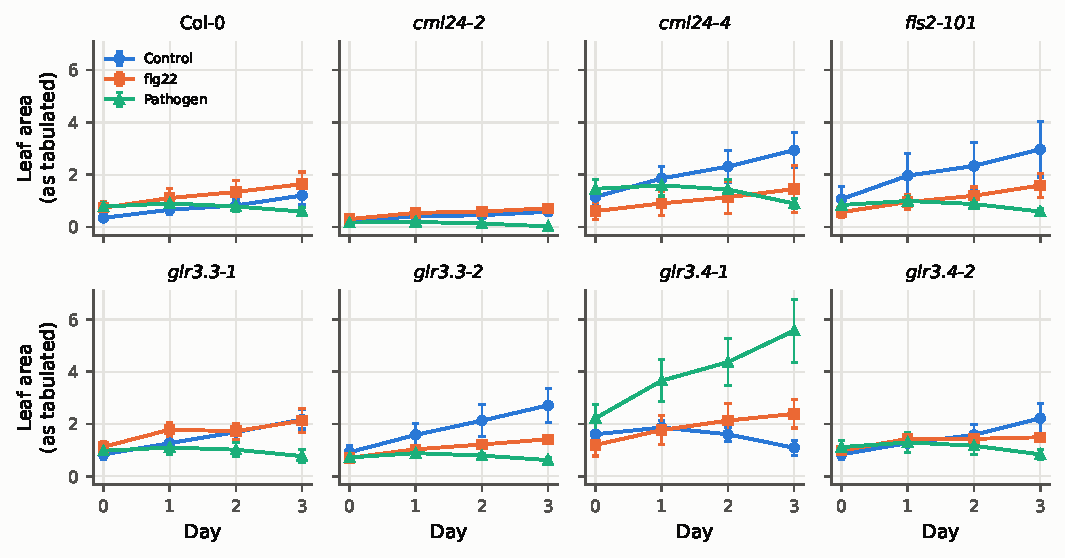
\includegraphics[width=\linewidth]{figS1_pilot_leaf_area.pdf}
\caption{Pilot (February--March 2016) leaf area, days 0--3. Values as tabulated in 2016; the
source sheet's second area column is 4$\times$ larger, and which is correct is unresolved (FACTS
R10, P12). Data: \texttt{tables/figS1\_pilot\_leaf\_area.csv}.}
\end{figure}

\section*{Supplementary Table: strongest baseline-adjusted contrasts}
% Generated by scripts/07_numbers.py
\begin{table}[ht]\centering\small
\caption{Baseline-adjusted contrasts with $p<0.01$ (set A; all 270 tests in tables/stats\_contrasts\_baseline\_adjusted.csv).}\label{tab:baseline}
\begin{tabular}{lllllll}
\toprule
Hour & Feature & Contrast & Effect (SD) & Effect (units) & $p$ & $q$ \\
\midrule
24 & shortwave\_fraction & Pathogen vs Control (Col-0) & 2.46 & 0.05944 & 1.6e-07 & 0.000 \\
2 & red\_fwhm\_nm & Pathogen vs Control (Col-0) & 2.39 & 1.762 & 5.0e-06 & 0.001 \\
3 & shortwave\_fraction & Pathogen vs Control (Col-0) & 2.03 & 0.0006432 & 7.6e-06 & 0.001 \\
24 & red\_fwhm\_nm & Pathogen vs Control (Col-0) & 2.23 & 3.348 & 7.4e-05 & 0.005 \\
3 & red\_fwhm\_nm & Pathogen vs Control (Col-0) & 2.07 & 1.017 & 9.8e-05 & 0.005 \\
3 & red\_fwhm\_nm & flg22 vs Control (Col-0) & 2.18 & 1.074 & 1.2e-04 & 0.005 \\
1 & red\_fwhm\_nm & Pathogen vs Control (Col-0) & 2.07 & 1.404 & 5.1e-04 & 0.018 \\
2 & shortwave\_fraction & Pathogen vs Control (Col-0) & 1.77 & 0.0004837 & 5.3e-04 & 0.018 \\
1 & farred\_fraction & Pathogen vs Control (Col-0) & 1.94 & 0.02878 & 1.2e-03 & 0.033 \\
2 & farred\_fraction & Pathogen vs Control (Col-0) & 1.86 & 0.02795 & 1.2e-03 & 0.033 \\
24 & shortwave\_fraction & Pathogen x cml24-4 & -1.74 & -0.042 & 1.4e-03 & 0.036 \\
48 & red\_fwhm\_nm & flg22 vs Control (Col-0) & 1.49 & 0.9618 & 1.7e-03 & 0.037 \\
2 & centroid\_nm & Pathogen vs Control (Col-0) & 1.82 & 1.667 & 2.3e-03 & 0.048 \\
1 & centroid\_nm & Pathogen vs Control (Col-0) & 1.88 & 1.706 & 2.7e-03 & 0.052 \\
2 & f685\_f740 & Pathogen vs Control (Col-0) & -1.74 & -0.8395 & 4.0e-03 & 0.073 \\
2 & red\_fwhm\_nm & flg22 vs Control (Col-0) & 1.60 & 1.177 & 4.4e-03 & 0.074 \\
1 & f685\_f740 & Pathogen vs Control (Col-0) & -1.75 & -0.8463 & 7.2e-03 & 0.114 \\
24 & shortwave\_fraction & Pathogen x cml24-2 & -1.41 & -0.03421 & 9.5e-03 & 0.132 \\
48 & farred\_fraction & flg22 vs Control (Col-0) & 1.29 & 0.01529 & 9.5e-03 & 0.132 \\
48 & f685\_f740 & flg22 vs Control (Col-0) & -1.26 & -0.5149 & 9.8e-03 & 0.132 \\
\bottomrule
\end{tabular}
\end{table}


\end{document}
